\documentclass[a4paper,11pt]{article}
\usepackage[verbose,a4paper,tmargin=2cm,bmargin=2cm,lmargin=2.5cm,rmargin=2.5cm]{geometry}
\usepackage[utf8]{inputenc}
\usepackage{polski}
\usepackage{amsmath}
\usepackage{amsfonts}
\usepackage{amssymb}
\usepackage{lastpage}
\usepackage{indentfirst}
\usepackage{verbatim}
\usepackage{graphicx}
\usepackage{fancyhdr}
\usepackage{listings}
\usepackage{hyperref} 
\usepackage{xcolor}
\usepackage{tikz}

\usepackage{array,multirow,graphicx}
\usepackage{float}

\frenchspacing
\pagestyle{fancyplain}
\fancyhf{}
\renewcommand{\headrulewidth}{0pt}
\renewcommand{\footrulewidth}{0.4pt}
\newcommand{\degree}{\ensuremath{^{\circ}}} 
\fancyfoot[L]{MI: Justyna Hubert 210200, Karol Podlewski 210294}
\fancyfoot[R]{\thepage\ / \pageref{LastPage}}


\begin{document}

\begin{titlepage}
\begin{center}
\begin{tabular}{rl}
\begin{tabular}{|r|}
\hline \\
\large{\underline{210200~~~~~~~~~~~~~~~~~~~~~~~~~~~~~~~~~~~~~~~~~~} }\\
$^{numer\ indeksu}$\\
\large {\underline{Justyna Hubert~~~~~~~~~~~~~~~~~~~~~~~~~~~~~~} }\\
$^{imie\ i\ nazwisko}$ \\\\ \hline
\end{tabular} 
&
\begin{tabular}{|r|}
\hline \\
\large{\underline{210294~~~~~~~~~~~~~~~~~~~~~~~~~~~~~~~~~~~~~~~~~~} }\\
$^{numer\ indeksu}$\\
\large {\underline{Karol Podlewski~~~~~~~~~~~~~~~~~~~~~~~~~~~~~~} }\\
$^{imie\ i\ nazwisko}$ \\\\ \hline
\end{tabular} 

\end{tabular}
~\\~\\~\\ 
\end{center}
\begin{tabular}{ll}
\LARGE{\textbf{Data}}& \LARGE{23.11.2019}\\
\LARGE{\textbf{Kierunek}}& \LARGE{Informatyka}\\
\LARGE{\textbf{Rok akademicki}}& \LARGE{2019/20} \\
\LARGE{\textbf{Semestr}}& \LARGE{7} \\
\LARGE{\textbf{Specjalizacja}}& \LARGE{IOAD} \\
\LARGE{\textbf{Grupa dziekańska}}& \LARGE{3} \\~\\~\\~\\~\\
\end{tabular}

\begin{center}
\textbf{\Huge{\\~\\Marketing Internetowy\\~\\~\\~\\~\\}}
\end{center}


\begin{center}
\textbf{\Large{Zadanie 2\\Wizytówka firmowa www }}
\textbf{\Huge{\\~\\Biuro architektoniczne}}	
\end{center}

\end{titlepage}
\setcounter{page}{2}


\section {Charakterystyka branży}

Biuro architektoniczne, które w obecnych chce zarabiać, musi mieć stronę internetową. Wciąż isteniają firmy, które zbierają projekty wielu architektów na jednym portalu, trudno jednak liczyć na porównywalny zysk, kiedy musimy się dzielić z pośrednikiem. Dlatego coraz więcej osób decyduje się na usamodzielnienie w tym aspekcie. Strona internetowa jest do tego kluczem.  \\

Większość stron jest zbudowana w prosty sposób, informując po krótce o architektach oraz pokazując przykładowe realizacje. Nie wyłamywaliśmy się z tego trendu.


\section {Technologie}

Tworząc stronę internetową biura architektonicznego wykorzystaliśmy technologie:

\begin{itemize}
    \item HTLM5
    \item CSS
    \item JavaScript
    \item Biblioteka Bootstarp 4
\end{itemize}

\section {Opis witryny}

Tworząc stronę biura architektonicznego zdecydowaliśmy się na zupełnie inne podejście, niż przy wcześniej porównywanej przez nas branży – treści ma być w tym wypadku mniej, nie trzeba więc tworzyć rozbudowanej witryny. Zdecydowaliśmy się na jeden plik HTML, w którym znajdą się wszystkie potrzebne informacje dla potencjalnego klienta. 

\subsection {Sekcja wstępna}

Sekcja ta zawiera kilka rotujących slajdów, które pokazują przykładowe relalizacje biura oraz napis zachęcający do przejrzenia strony.  \\

\begin{figure}[H]
	\centering
	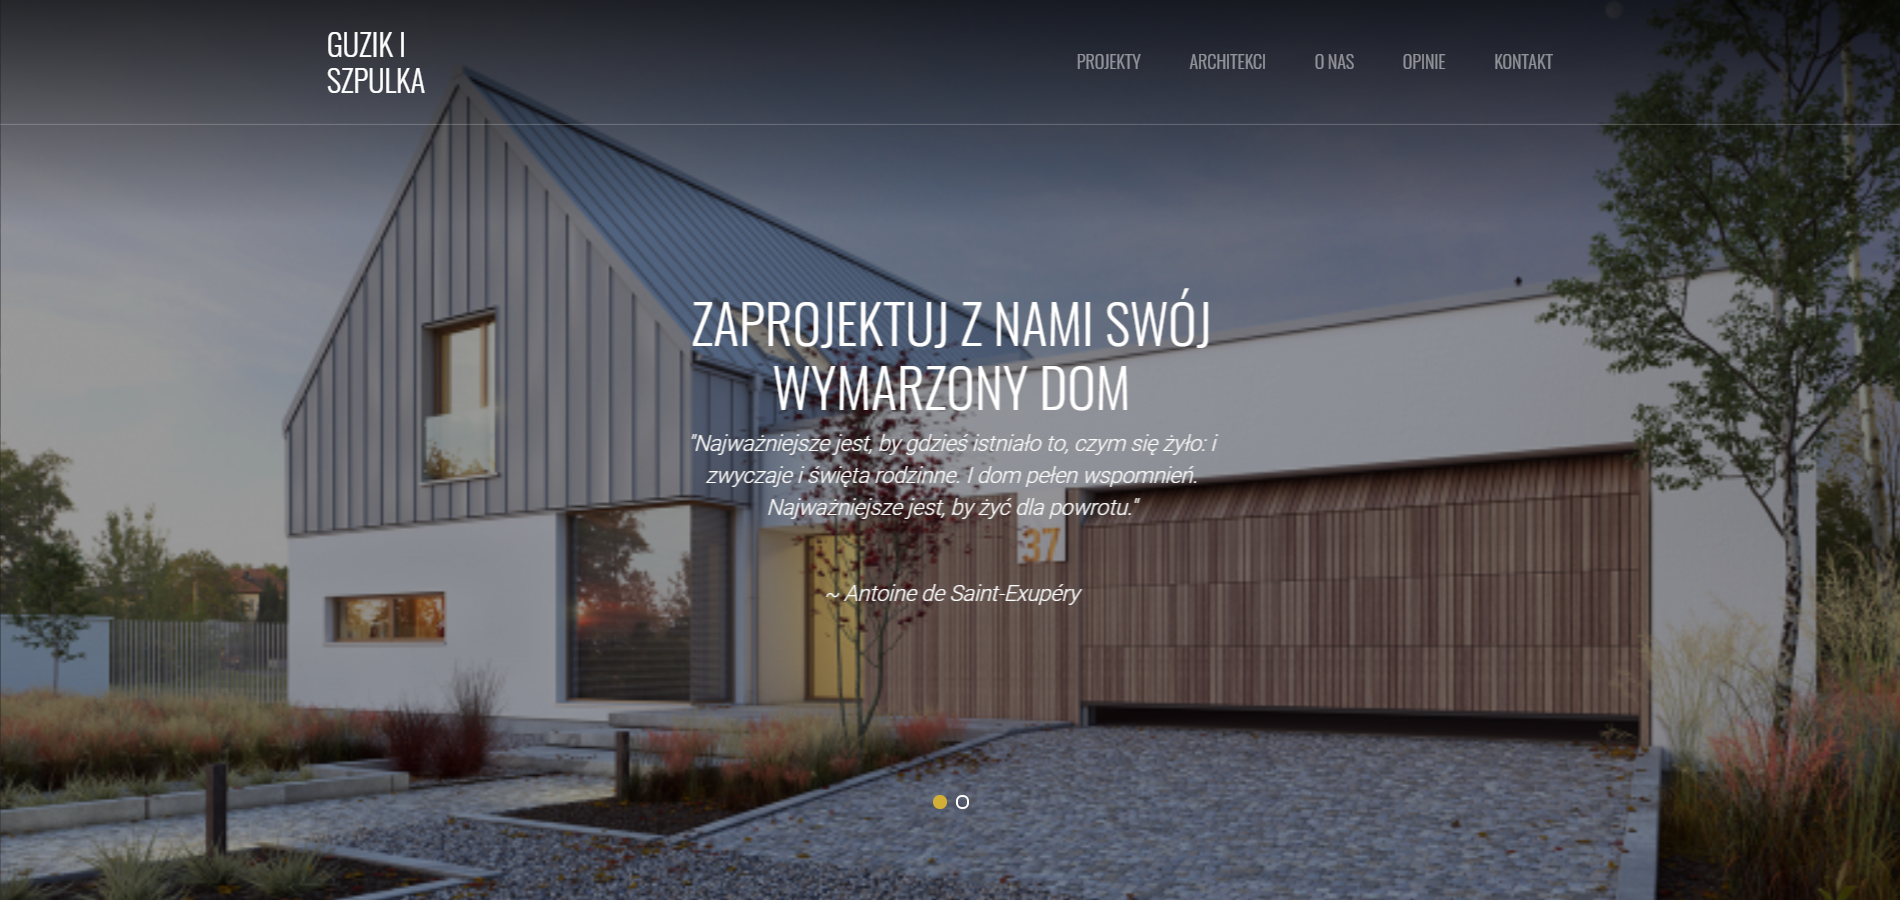
\includegraphics[width=1\textwidth]{{Zdjecia/0.png}}
	\caption{Sekcja wstępna}
\end{figure}


\subsection {Projekty}

Pokazane są tutaj wyróżniające się projekty przygotowane przez biuro architektoniczne wraz z krótką informacją na ich temat.  \\

\begin{figure}[H]
	\centering
	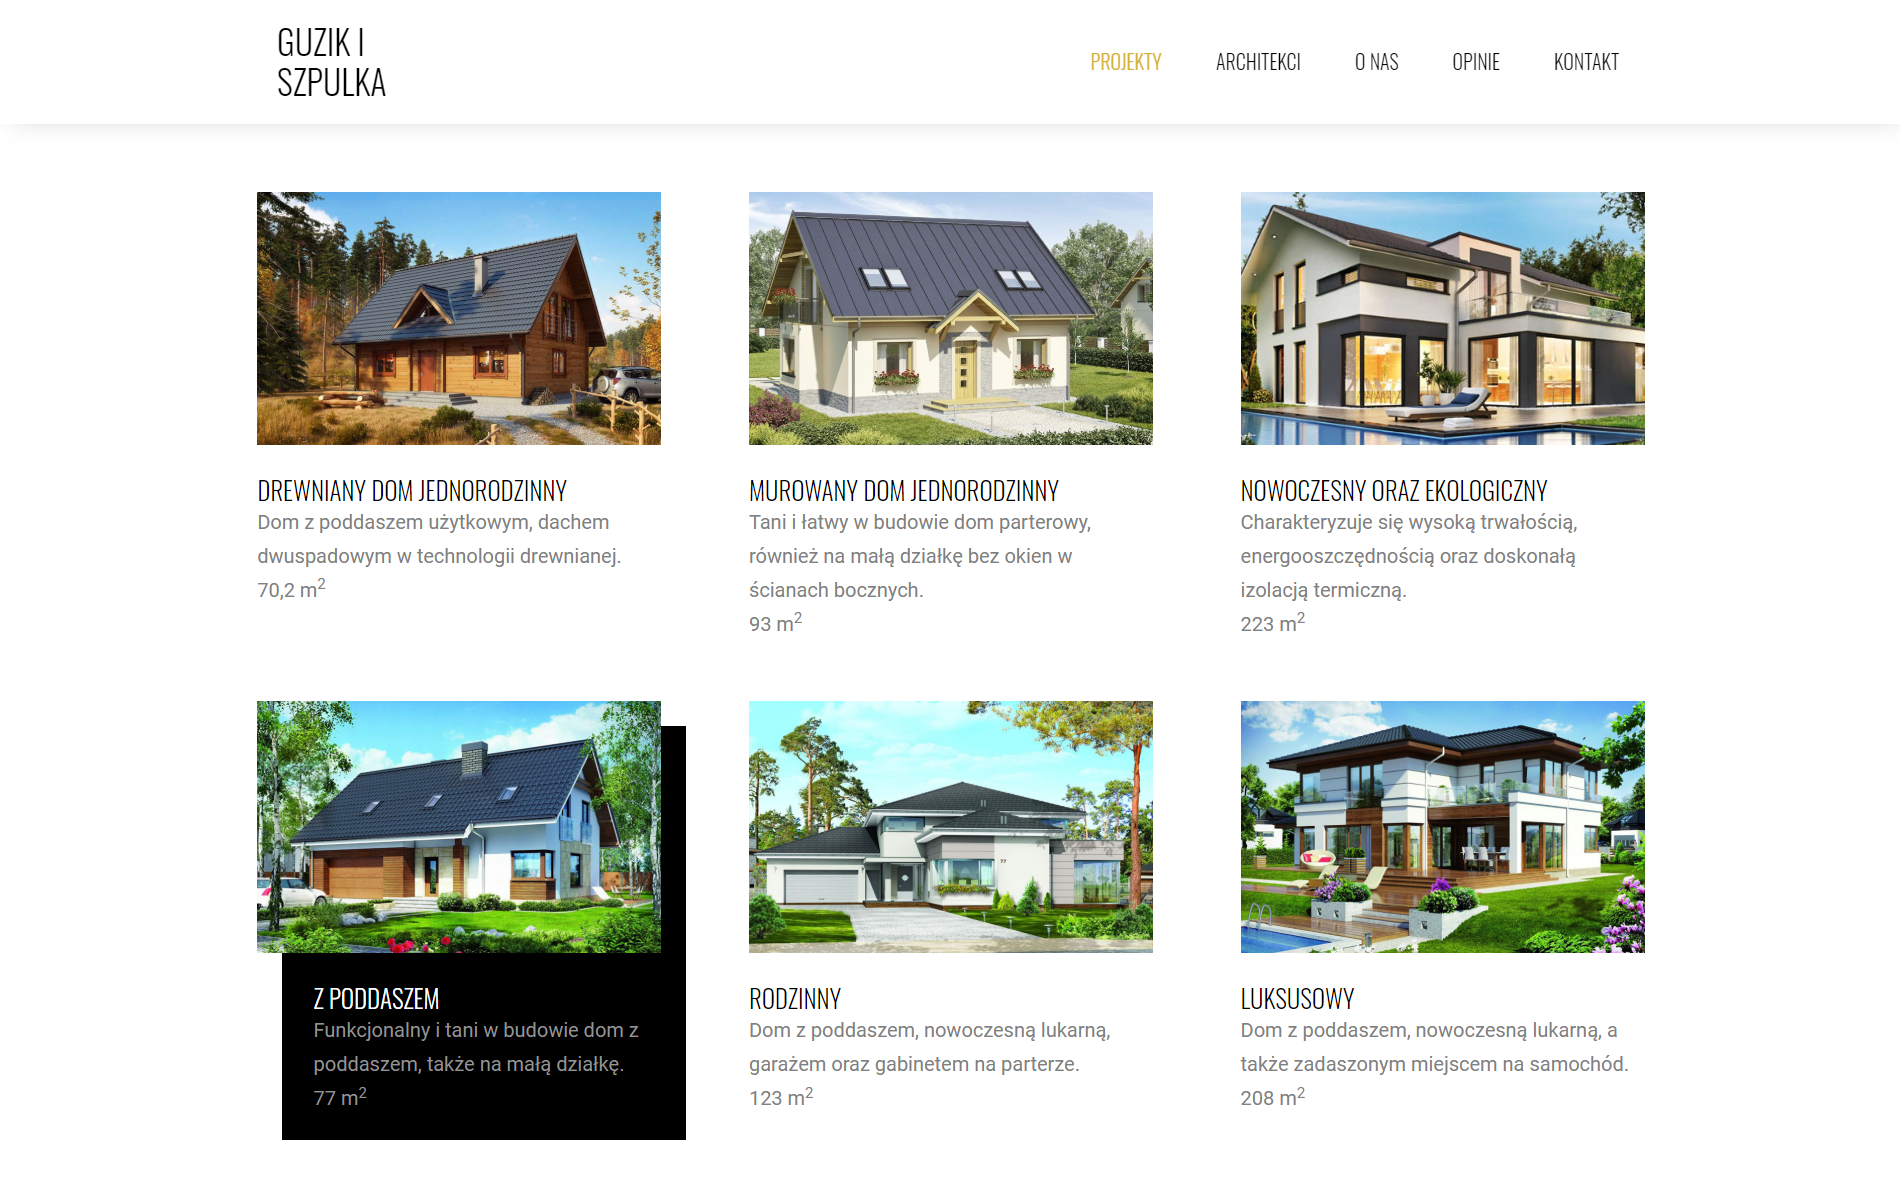
\includegraphics[width=1\textwidth]{{Zdjecia/1.png}}
	\caption{Sekcja projektów}
\end{figure}

\subsection {Architekci}

W tej sekcji pokazani są architekci pracujący dla biura, wraz z linkami do ich mediów społecznościowych (m.in. linkedin).  \\


\begin{figure}[H]
	\centering
	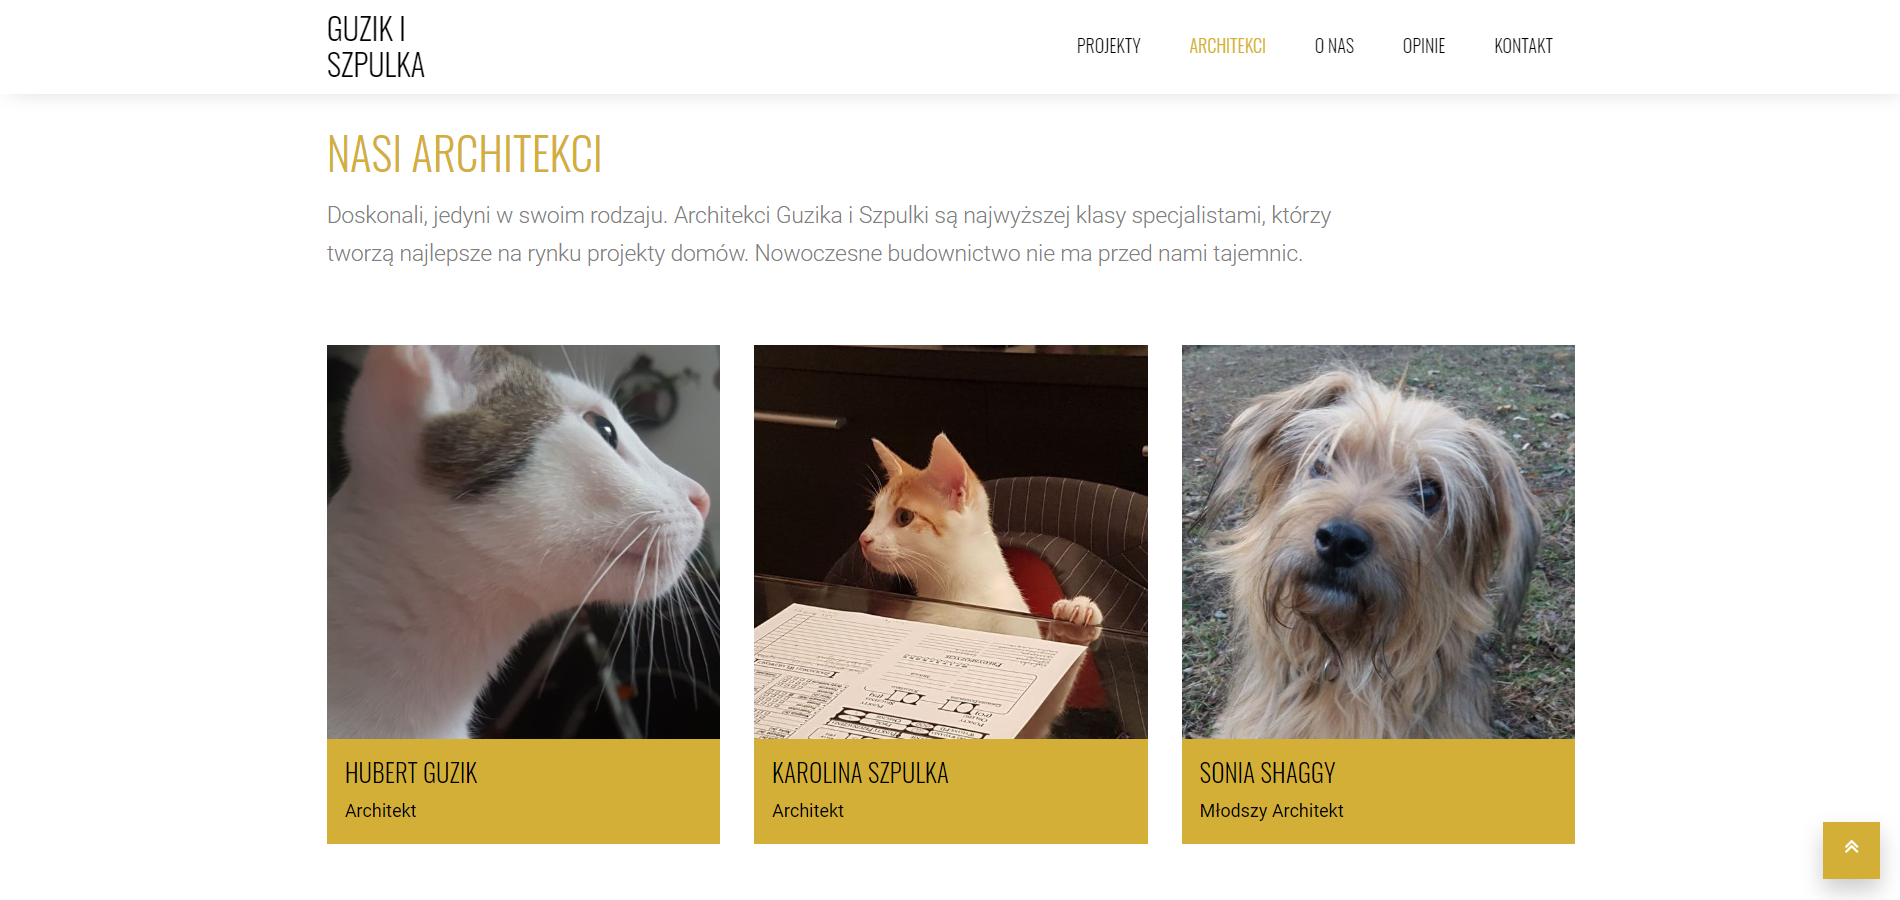
\includegraphics[width=1\textwidth]{{Zdjecia/2.png}}
	\caption{Sekcja architektów}
\end{figure}


\subsection {O nas}

Krótki opis pracowników, których można zobaczyć przy pracy i poznać z bardziej ludzkiej strony.  \\

\begin{figure}[H]
	\centering
	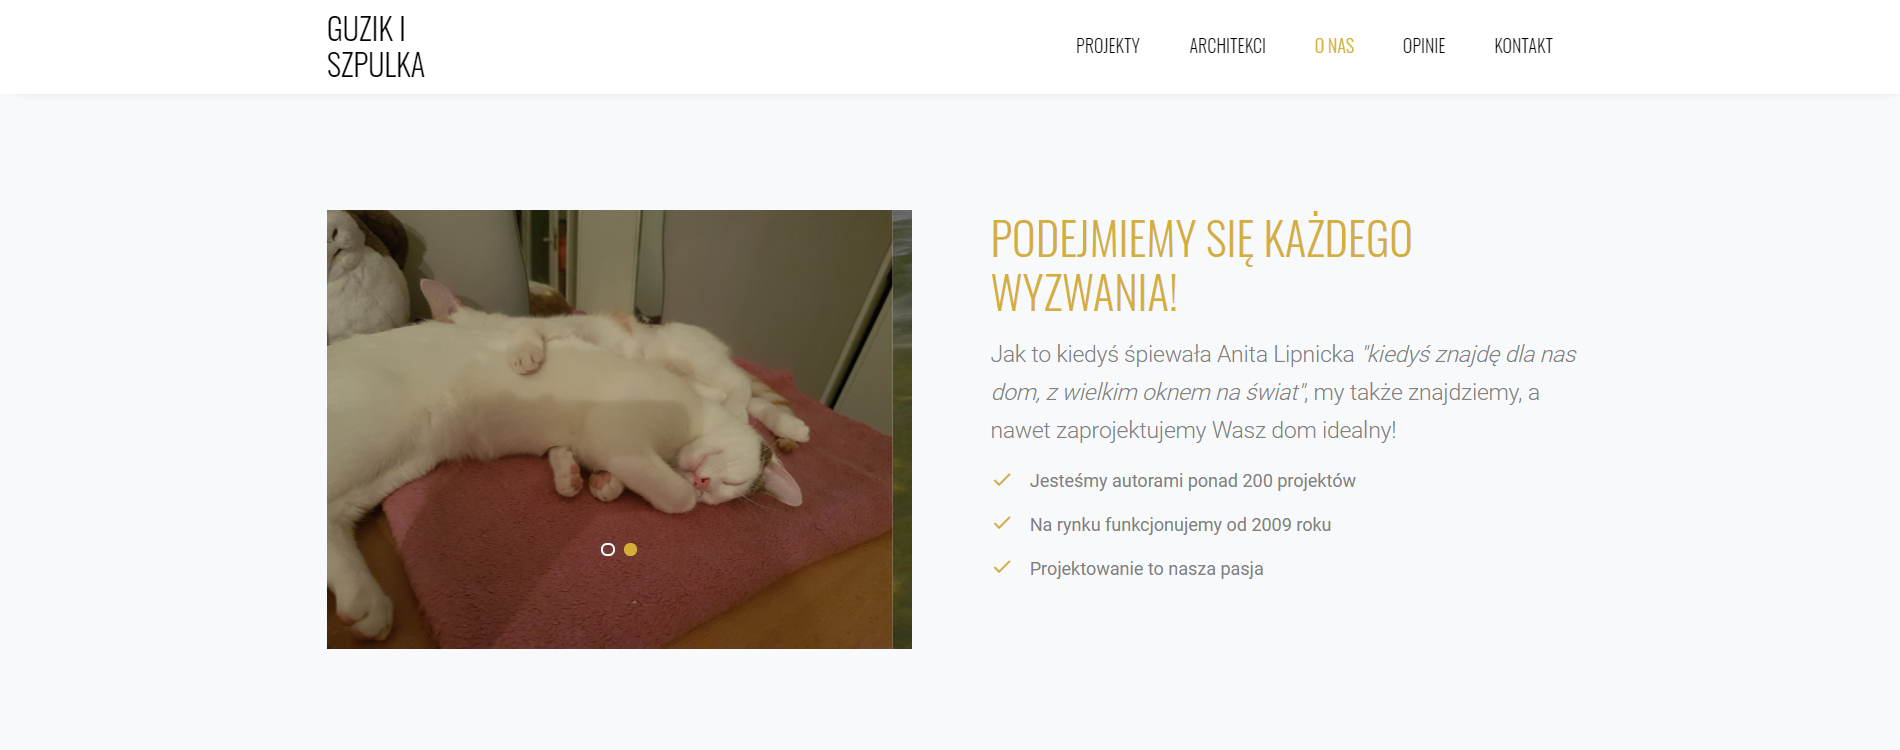
\includegraphics[width=1\textwidth]{{Zdjecia/3.png}}
	\caption{Sekcja "O nas"}
\end{figure}


\subsection {Opinie}

W tej sekcji przedstawione są niedawne opinie znanych ludzi, które potwierdzają jakość biura architektonicznego.  \\

\begin{figure}[H]
	\centering
	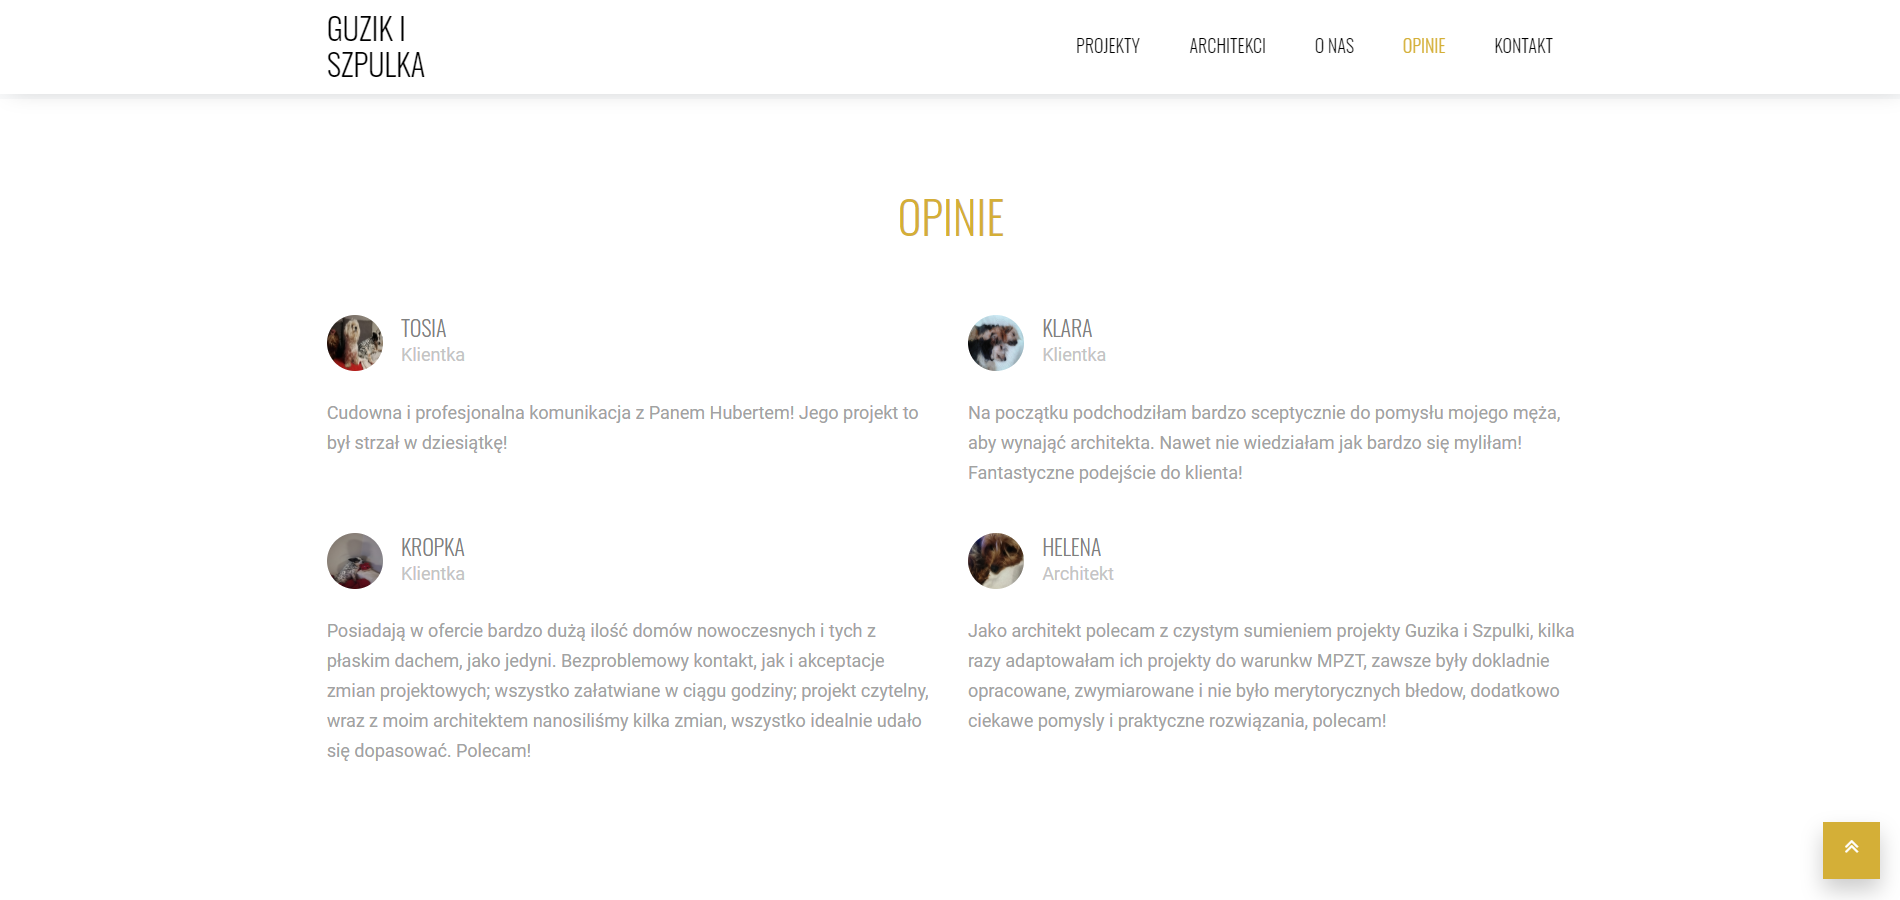
\includegraphics[width=1\textwidth]{{Zdjecia/4.png}}
	\caption{Sekcja opinii}
\end{figure}



\subsection {Kontakt}

W sekcji konktatkowej umieściliśmy podstawowe informacje potrzebne do kontaktu w przypadku chęci skorzystania z usług biura, m.in adres, numer telefonu czy email a także możliwośc kontaktu bezpośrednio ze strony za pomocą przygotowanego formularza.  \\

\begin{figure}[H]
	\centering
	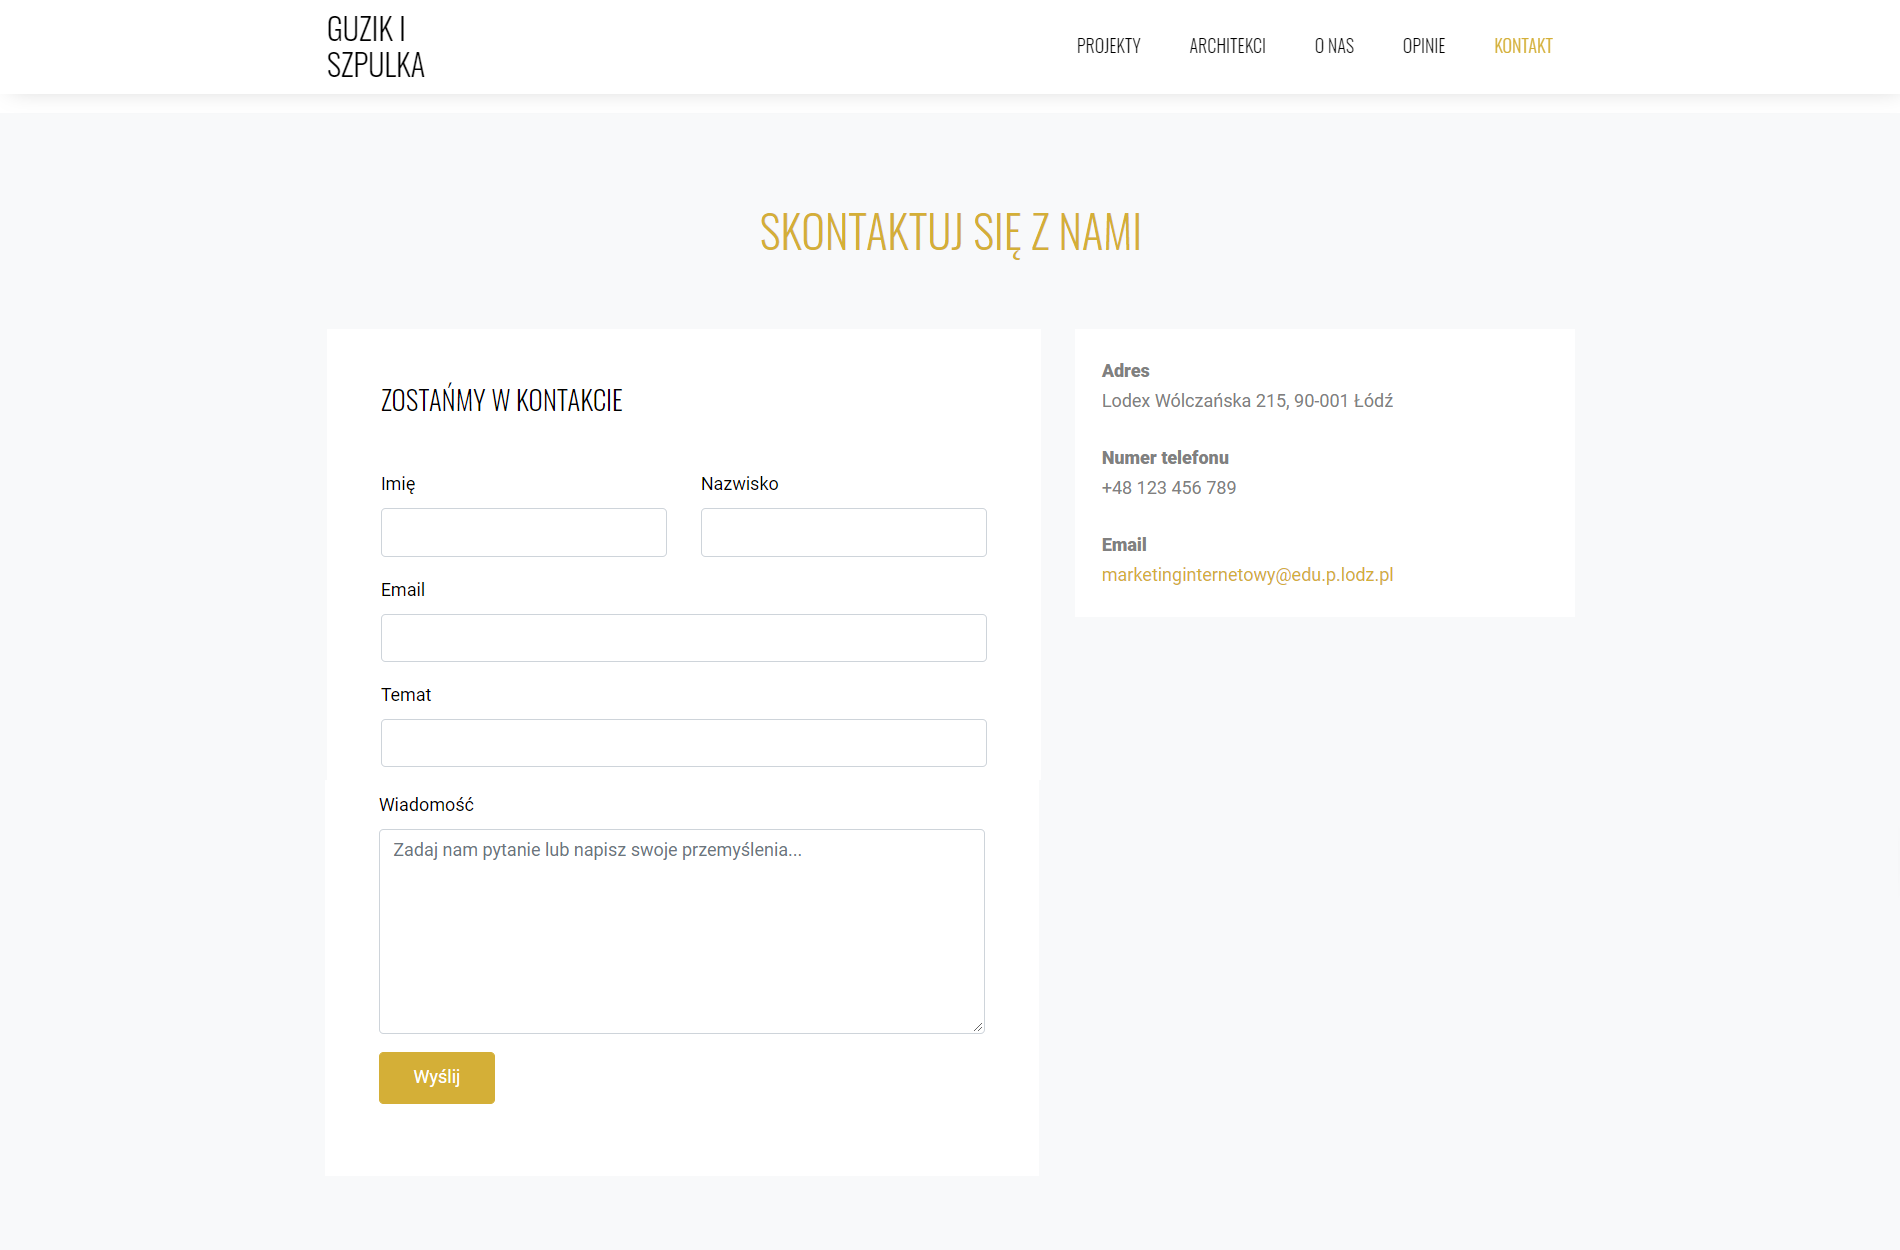
\includegraphics[width=1\textwidth]{{Zdjecia/5.png}}
	\caption{Sekcja kontaktowa}
\end{figure}


\subsection {Stopka}

Prosta stopka z możliwością zapisania się do newslettera oraz śledzenia mediów społecznościowych.  \\

\begin{figure}[H]
	\centering
	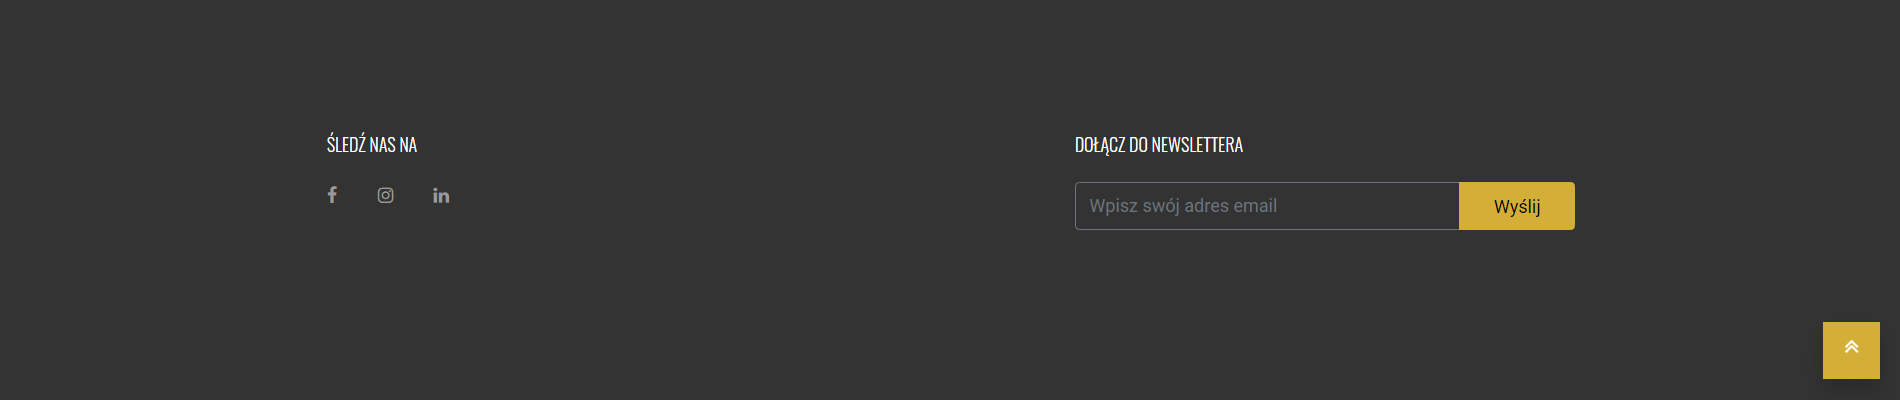
\includegraphics[width=1\textwidth]{{Zdjecia/6.png}}
	\caption{Stopka}
\end{figure}

\section {Wnioski}
\begin{itemize}
	\item Użycie biblioteki Bootsrtap znacznie przyśpieszyło pracę nad stroną-wizytówką. Przy niewielkim nakładzie pracy udało nam się stworzyć profesjonalnie wyglądającą witrynę. 
	\item Porównywanie witryn w 1 etapie w wielu aspektach było uniwersalne, co pomogło nam stworzyć lepszą stronę.
	\item Dużej części wyciągniętych wniosków z 1 etapu nie byliśmy w stanie zastosować podczas tworzenia strony w zupełnie innej branży.
	\item Wiele z biur architektonicznych przykłada zbyt dużą uwagę do wyglądu strony, nie zwracając uwagi na funckjonalność tak prostych witryn. W branży gier fabularnych tendencja była odwrotna.
\end{itemize} 

\end{document}